\documentclass[12pt]{article}

\usepackage[margin=1.9cm, letterpaper]{geometry}
\usepackage[utf8]{inputenc}
\usepackage{indentfirst}
\usepackage{tikz}
\usepackage{float}
\usepackage{subcaption}
\usepackage{amsmath}
\usepackage{amssymb}
\usepackage{booktabs}
\usepackage{siunitx}
\usepackage{pdfpages}
\usepackage[outputdir=obj]{minted}
\usepackage{fontspec}
\usepackage{hyperref}

\setmainfont{Noto Serif}
\setsansfont{Segoe UI}
\setmonofont{Consolas}

% \usemintedstyle{monokai}
% \definecolor{codeBg}{HTML}{282822}
% \setminted{bgcolor=codeBg}

\usetikzlibrary{arrows,automata,positioning}

\begin{document}
\begin{titlepage}
  \begin{center}
    \vspace*{1cm}

    \textbf{LAB 3}

    \vspace{0.5cm}

    8-bit CPU

    \vspace{1.5cm}

    \textbf{Michael Kwok (1548454)}

    \vfill

    ECE 410 -- Advanced Digital Logic Design\\
    Department of Electrical and Computer Engineering\\
    University of Alberta\\
    October 20, 2021

  \end{center}
\end{titlepage}

\tableofcontents

\pagebreak

\section{Abstract}

In this lab, a simple non-pipelined 8-bit CPU was designed. For this, a design using both a datapath and controller was used. The datapath was designed with the structural method, then the controller was designed using the behavioural method, with signals between the datapath and controller to control what the datapath should do and for the datapath to signal the controller about the status.

The Zybo board was used for implementation, and peripheral devices such as the Seven Segment Display, LEDs and Switches were used to control the CPU.

\section{Design}

To simplify the CPU, a load store accumulator design was used. The CPU was designed with the datapath modelling technique, where the sequential logic device is designed with two related modules, the datapath and the controller. The datapath is combinational logic that handles the data, while the controller controls the what the datapath needs to do.

\subsection{Datapath}

\begin{figure}[H]
  \centering
  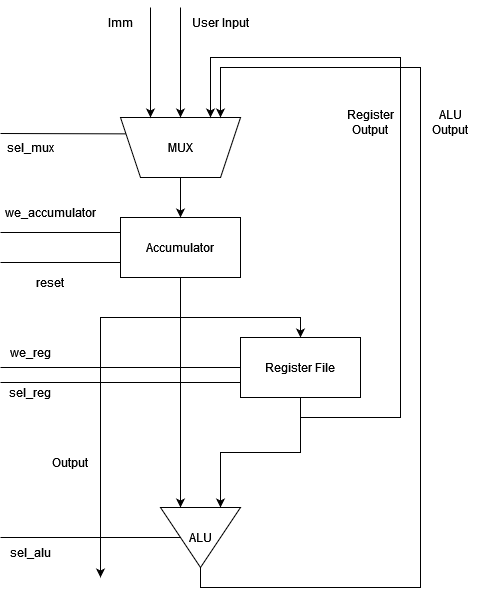
\includegraphics[width=0.5\linewidth]{datapath.png}
  \caption{Datapath Flowchart}
  \label{fig:datpath-diagram}
\end{figure}

The datapath is designed structurally, which is where each component is instantiated in the datapath module, then connected to each other via signals. A 4 to 1 MUX was used to handle inputs into an accumulator which is connected to a register file, an ALU and the output.

\subsection{Controller}

The controller used the behavioural technique for modelling, as it was simpler to implement. The three stages of execution for a CPU are the Fetch, Decode and Execute stages. A where-case construct was used to implement the stages. In the Execute stage, another where-case construct was used to implement each instruction again. This causes each instruction to take three clock cycles to complete as the CPU is not pipelined.

In each state, the correct control signals are asserted, and the PC is modified appropriately to keep the processor running.

\section{Testing \& Simulation}

The design was tested with two programs. The input for both programs are set to be \verb|1101|

Program 1:
\begin{verbatim}
  IN A
  IN A
  JZ 05
  SHFL A
  OUT A 
  LDI A, 10
  SHFR A
  OUT A
  HALT
\end{verbatim}

\begin{figure}[H]
  \centering
  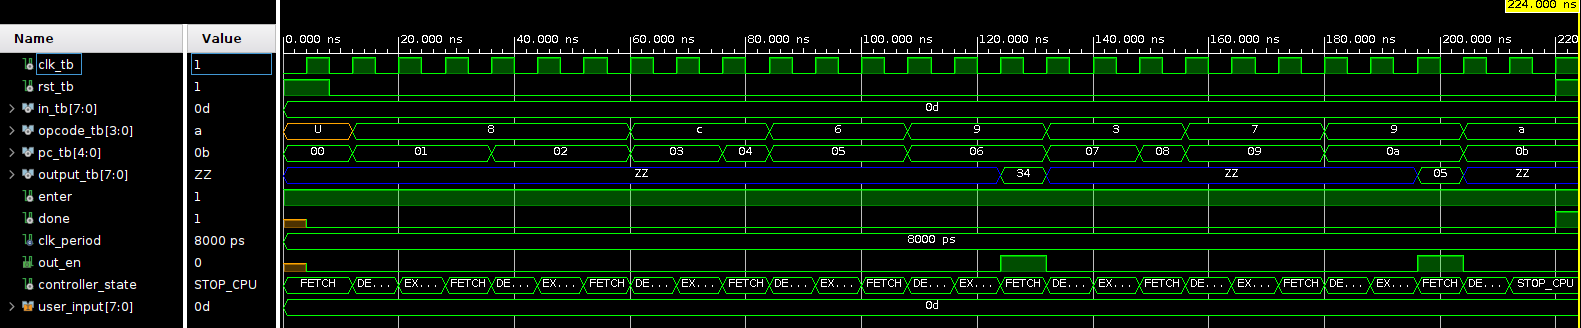
\includegraphics[width=\linewidth]{Program1_waveform.png}
  \caption{Program 1 Waveform}
\end{figure}

Program 2:
\begin{verbatim}
  IN A
  IN A
  STA R4, A
  LDI A, 15
  ADD A, R4
  OUT A
  HALT
\end{verbatim}

\begin{figure}[H]
  \centering
  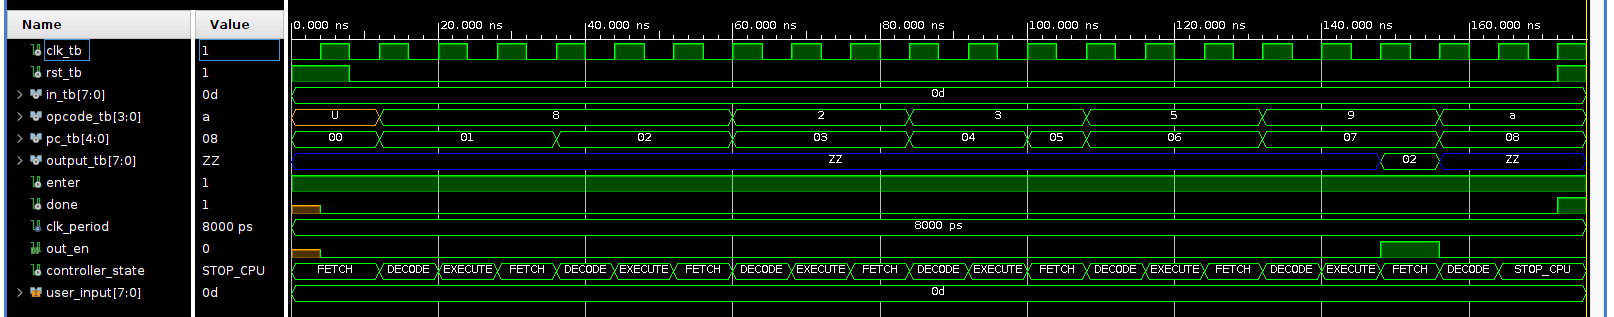
\includegraphics[width=\linewidth]{Program2_waveform.png}
  \caption{Program 2 Waveform}
\end{figure}

\section{Conclusion}

In this lab, a simple CPU with an accumulator load-store architecture was designed as an exercise to implement a datapath. The importance of designing the datapath before the controller was shown as a device this complex has many signals that needs to be shared between the two modules.

% \section{References}
\pagebreak
\section{Appendix}

\subsection{Top Level File}
\inputminted{vhdl}{../src/Lab3_top.vhd}

\pagebreak
\subsection{Clock Divider}
\inputminted{vhdl}{../src/ClockDivider.vhd}

\pagebreak
\subsection{Control Unit}
\inputminted{vhdl}{../src/ControlUnit.vhd}

\pagebreak
\subsection{CPU Core}
\inputminted{vhdl}{../src/CpuCore.vhd}

\pagebreak
\subsection{Program Memory}
\inputminted{vhdl}{../src/ProgMem.vhd}

\pagebreak
\subsection{Seven Segment Decoder}
\inputminted{vhdl}{../src/SevenSegmentDecoder.vhd}

\pagebreak
\subsection{Datapath}
\inputminted{vhdl}{../src/datapath/Datapath.vhd}

\pagebreak
\subsection{Accumulator}
\inputminted{vhdl}{../src/datapath/Accumulator.vhd}

\pagebreak
\subsection{ALU}
\inputminted{vhdl}{../src/datapath/ALU.vhd}

\pagebreak
\subsection{4 to 1 MUX}
\inputminted{vhdl}{../src/datapath/MUX4.vhd}

\pagebreak
\subsection{Register File}
\inputminted{vhdl}{../src/datapath/RegisterFile.vhd}

\pagebreak
\subsection{Tristate Buffer}
\inputminted{vhdl}{../src/datapath/TristateBuffer.vhd}

\end{document}
